
\chapter{Linguagens Livres do Contexto}\label{cap:LinguagemLLC}

\begin{introduction}[Conteúdos]
	\item Gramática Livres do Contexto
	\item Simplificação e Formas Normais de GLC
	\item Autômato de Pilha Determinístico
	\item Autômato de Pilha Não-determinístico
	\item Álgebra das Linguagens Livres de Contexto
	\item Questionário
\end{introduction}

No capítulo passado foram apresentadas três diferentes formalismos para a classe das linguagens regulares, a saber, o formalismo operacional (os autômatos), o formalismo denotacional (as expressões regulares) e por fim o formalismo gerador ou axiomático (as gramáticas regulares). Agora este manuscrito irá continuar o estudo das linguagens formais apresentando a classe das linguagens livres do contexto, como antes serão apresentados diferentes formalismo para tal classe de linguagens.

\section{Gramática Livres do Contexto}\label{sec:GLC}

O estudo das Linguagens Livres do Contexto será iniciado aqui pela apresentação de seu formalismo gerador, ou seja, será primeiro apresentado a noção de Gramática Livre do Contexto.

\begin{definition}[Gramática Livre do Contexto]\label{def:GLC}
	\cite{benjaLivro2010} Uma Gramática Livre do Contexto, ou simplesmente GLC, é uma gramática formal $G = \langle V, \Sigma, S, P\rangle$ onde todo $\alpha \rhd \beta \in P$ é tal que $\alpha \in V$ e $\beta \in (V \cup \Sigma)^*$.
\end{definition}

\begin{example}\label{exe:GLC-1}
	A estrutura $G = \langle \{A, B, C\}, \{0,1\}, A, P\rangle$ onde $P$ é definido pela regras:
	\begin{eqnarray*}
		A & \rhd & A0110BC \mid 0110C \mid AAB0110CC \mid \lambda\\
		B & \rhd & 01B10 \mid 0110\\
		C & \rhd & 01C \mid \lambda
	\end{eqnarray*}
	é uma GLC.
\end{example}

Obviamente o leitor atento pode notar que a Definição \ref{def:GLC} garante que toda Gramática Regular é um caso particular de GLC, porém o inverso não é verdadeiro, basta notar que a gramática apresentada no Exemplo \ref{exe:GLC-1}, fere a definição de gramática regular apresentada na Seção \ref{sec:GramaticaRegular} do capítulo passado. Agora utilizando a Definição \ref{def:LinaugemGramatica} pode-se formalizar o conceito de Linguagem Livre do Contexto.

\begin{definition}[Linguagem Livre do Contexto]\label{def:LLC}
	A linguagem $L$ gerada por uma GLC $G$, ou seja, $L = \mathcal{L}(G)$, será chamada de Linguagem Livre do Contexto, ou simplesmente LLC.
\end{definition}

Como para os casos das linguagens reconhecidas por AFD, para provar que uma determinada GLC $G$ gera uma linguagem $L$ é necessário demonstrar o seguinte resultado $w \in L \Longleftrightarrow w \in \mathcal{L}(G)$.

\begin{example}\label{exe:LinguagemGLC}
	A linguagem $L = \{a^ib^i \mid i  > 0\}$ é gerado pela GLC $G = \langle \{S\}, \{a,b,c\}, S, P\rangle$ onde $P$ é formado pelas regras,
	\begin{eqnarray*}
		S & \rhd & aSb \mid ab
	\end{eqnarray*}
	\begin{proof}
		$(\Rightarrow)$ Suponha que $w \in L$ assim $w = a^ib^i$ para $i  > 0$, agora por indução sobre a quantidade $n$ de derivações em $G$ será mostrado que toda forma sentencial gerada por $G$ é da forma $a^nS^jb^n$ com $j \in \{0, 1\}$. 
		\begin{itemize}
			\item[ ] \textbf{Base da indução}: Com $n = 1$, é trivial pelas regras em $P$. 
			\item[ ] \textbf{Hipótese indutiva (HI)}: Assuma que com $n$ derivações tal que $n \geq 0$ a forma sentencial $a^nS^jb^n$ é gerada pela GLC $G$, ou seja, $S \gg^n a^nS^jb^n$ com $j \in \{0, 1\}$. 
			\item[ ] \textbf{Passo indutivo}: Agora dado $S \gg^{n+1} w'$, ou seja, $w'$ é derivada de $S$ com $n+1$ derivações, assim por definição tem-se que existe $w''$ tal que $S \gg^n w'' \gg w'$, mas por \textbf{(HI)} tem-se que $w'' =  a^nS^jb^n$ com $n \geq 0$ e $j \in \{0, 1\}$,  desde que, $w'$ é gerada de $w''$ é claro que $j = 1$, ou seja, $w'' = a^nSb^n$, consequentemente, $w' = a^{n+1}Sb^{n+1}$ ou $w' = a^{n+1}b^{n+1}$ e, portanto, $w'$ é da forma $a^{n+1}S^jb^{n+1}$ com $j \in \{0, 1\}$. 
		\end{itemize}
		Agora por hipótese tinha-se que $w = a^ib^i$ para $i  > 0$, ou seja, $w = a^iS^0b^i$, dessa forma pela indução acima $w$ é uma forma sentencial gerada por $G$, e como $w \in \Sigma^*$ tem-se por definição que $w \in \mathcal{L}(G)$. $(\Rightarrow)$ Suponha que $w \in \mathcal{L}(G)$, agora será mostrado por indução sobre a quantidade $n$ de derivações que todo $w$ gerado por $G$ estará em $L$.
		\begin{itemize}
			\item[ ] \textbf{Base da indução:} Com $n=1$, ou seja, como uma única derivação, pelo fato de que $w \in \Sigma^*$ e pelas regras em $P$ tem-se obrigatoriamente que $w = ab$ e, portanto, $w = a^1b^1$ , consequentemente, $w \in L$.
			\item[ ] \textbf{Hipótese indutiva (HI)}: Assuma que para todo $S \gg^n w$ tal que $n \geq 1$, tem-se que $w \in L$.
			\item[ ] \textbf{Passo indutivo}: Agora dado $S \gg^{n+1} w$, ou seja, $w$ é derivado em $G$ com $n + 1$ derivações de forma que $n \geq 1$. Desde que $n  \geq 1$ tem-se que $n + 1  > 1$, assim a palavra $ab$ não pode ser $w$ uma vez que são usadas pelo menos duas derivações para gerar $w$. Assim a derivação de $w$ deverá ter sido iniciado usando a regra $S \rhd aSb$ e, portanto, $w = aw'b$ em que $S \gg^n w'$, mas pela hipótese indutiva $w' \in L$, logo $w' = a^ib^i$ com $i > 0$, consequentemente $w = aa^ib^ib = a^{i+1}b^{i+1}$, logo $w \in L$.
		\end{itemize}
	\end{proof}
\end{example}

Note que para a prova mostrada no Exemplo \ref{exe:LinguagemGLC} foi-se usada indução sobre o tamanho das derivações, isto não é a única forma de se proceder para provar que uma gramática gera uma determinada linguagem, de  fato como apresentado em \cite{hopcroft2008} pode-se usar a ideia de indução sobre as árvores de derivações (apresentadas mais a frente), neste manuscrito não será apresentado tal estratégia, porém fica a referência para interessados no tema. 

Nas GLC que não são lineares, ou seja, as gramática em que as regras em $P$ podem conter duas ou mais variáveis do lado direto do símbolo $\rhd$, é permitido a escolha sobre qual variável ser derivada primeiramente, para ilustrar isso considere uma forma sentencial $0A10BC$ e as regras $A \rhd 00, B \rhd \lambda$ e $C \rhd 1$, note que dependendo de qual variável é escolhida para ser reescrita a próxima forma sentencial pode assumir três formas diferentes. Apresentado esta ideia pode-se agora formalizar o conceito de reescrita \textbf{mais à esquerda} e \textbf{mais à direita}.

\begin{definition}[Tipos de Derivação]\label{def:TiposLateraisReescrita}
	Dado uma GLC $G = \langle V, \Sigma, S, P\rangle$ e seja $w_1A_1w_2\cdots w_nA_nw_{n+1}$ uma forma sentencial derivável em $G$ tal que $w_i \in \Sigma^*$ e $A_j \in V$ para todo $1 \leq i \leq n+1$ e $1 \leq j \leq n$. Uma derivação é dita mais à esquerda (à direita) se ela é da forma $w_1A_1w_2\cdots w_nA_nw_{n+1} \gg w_1w'w_2\cdots w_nA_nw_{n+1}$ ($w_1A_1w_2\cdots w_nA_nw_{n+1} \gg w_1A_1w_2\cdots w_nw'w_{n+1}$)  com  $w' \in (V \cup \Sigma)^*$.
\end{definition}

\begin{example}\label{exe:ReescritasLaterais}
	Considere a GLC $G = \langle \{S, A, B\}, \{0, 1\}, S, P\rangle$ em que $P$ é formado pelas regras,
	\begin{eqnarray*}
		S & \rhd & 0AB\\
		A & \rhd & 11B1 \\
		B & \rhd & A \mid \lambda 
	\end{eqnarray*}
	claramente a palavra $011B1A$ é um forma sentencial derivável em $G$, agora note que:
	\begin{eqnarray*}
		011B1A & \gg & 011A1A\\
		011B1A & \gg & 0111A
	\end{eqnarray*}
	são ambas derivações mais à esquerda, e 
	\begin{eqnarray*}
		011B1A & \gg & 011B111B1
	\end{eqnarray*}
	é uma derivação mais à direita.
\end{example}

\begin{definition}[Tipo de Geração]\label{def:TipoGeracao}
	Dado uma GLC $G = \langle V, \Sigma, S, P\rangle$,  uma derivação $S \gg^* w$ é dita ser uma geração mais à esquerda (à direita) sempre que $w \in \Sigma^*$ e toda derivação realizada for mais à esquerda (à direita).
\end{definition}

\begin{example}\label{exe:TipoGeracao}
	Considere a gramática do Exemplo \ref{exe:ReescritasLaterais} a derivação, 
	$$S \gg 0AB \gg 011B1B \gg 0111B \gg 0111$$
	é claramente uma geração mais à esquerda, já a derivação
	$$S \gg 0AB \gg 0A \gg 011B1 \gg 0111$$
	é notavelmente uma geração mais à direita.
\end{example}

\begin{remark}
  Resumindo dado uma uma GLC $G = \langle V, \Sigma, S, P\rangle$ uma geração é obrigatoriamente uma derivação $S \gg w$ em que $w \in \Sigma^*$, ou seja, uma derivação que gera (ou produz) uma palavra sobre o alfabeto $\Sigma$.
\end{remark}

Além da noção de geração, para visualizar o passo a passo da ``construção'' de uma palavra $w \in \Sigma^*$ em uma GLC $G$ é comum usar a ideia de árvore de derivação\footnote{Na literatura como no livro \cite{benjaLivro2010} também é comum encontrar a nomenclatura árvore ordenada.}. Uma árvore de derivação nada mais é do que uma forma visual estruturada em uma árvore que representar a construção de uma palavra, em que cada nível da árvore representa é gerada pela aplicação de uma ou mais regras de reescrita, neste sentido as folhos da árvore contém os símbolos da palavra $w$.

\begin{definition}[Árvore de Derivação]\label{def:ArvoreGLC}
	Seja $G = \langle V, \Sigma, S, P\rangle$ uma GLC e dado $w \in \mathcal{L}(G)$, uma árvore de derivação para $w$ é construída seguindo as seguintes regras:
	\begin{enumerate}
		\item O símbolo $S$ é a raiz da árvore.
		\item Todo símbolo $a \in \Sigma \cup \{\lambda\}$ é o rótulo de uma folha.
		\item Todo símbolo $A \in V$ é o rótulo de uma raiz de uma sub-árvore\footnote{Aqui sub-árvore e no mesmo sentido que o leitor já deve ter visto em estrutura de dados.}.
		\item Se $A$ é uma raiz e seus ``filhos'' são  $x_1, \cdots, x_n$ com $x_i \in V \cup \Sigma \cup \{\lambda\}$ para $1 \leq i \leq n$, então existe em $P$ uma regra da forma $A \rhd x_1\cdots x_n$.
		\item Todo folha rotulada por $\lambda$ de uma raiz $A$ será filho único, ou seja, em $P$ existe uma regra da forma $A \rhd \lambda$.
	\end{enumerate}
\end{definition}

\newpage
\begin{example}\label{exe:ArvoreGLC1}
	Tem-se que a derivação $S \gg 0AB \gg 011B1B \gg 0111B \gg 0111$ apresentada no Exemplo \ref{exe:TipoGeracao} é representada pela árvore esboçada na Figura \ref{fig:ArvoreGLC1} a seguir.
	
	\begin{figure}[h]
		\centering
		\begin{tikzpicture}[sibling distance=.6cm, empty/.style={draw=none}, tlabel/.style={font=\footnotesize\color{red!70!black}}]
			\Tree   [.$S$  
					[.$0$ ]
						%\edge node[tlabel,auto=left] {1}; 
					[.$A$  
							[.$1$ ]
							[.$1$ ]
							[.$B$ 
								{$\lambda$}
							] 
							[.$1$ ]
					] 
					[.B   
						%\edge[empty]; {} \edge node[tlabel,auto=left] {5}; {b}   
						{$\lambda$}
					]
			]
		\end{tikzpicture}
		\caption{Árvore para a derivação $S \gg 0AB \gg 011B1B \gg 0111B \gg 0111$.}
		\label{fig:ArvoreGLC1}
	\end{figure}
\end{example}

\begin{example}\label{exe:ArvoreGLC2}
	Tem-se que a derivação $S \gg 0AB \gg 0A \gg 011B1 \gg 0111$ apresentada no Exemplo \ref{exe:TipoGeracao} é representada pela árvore esboçada na Figura \ref{fig:ArvoreGLC2} a seguir.
	
	\begin{figure}[h]
		\centering
		\begin{tikzpicture}[sibling distance=.6cm, empty/.style={draw=none}, tlabel/.style={font=\footnotesize\color{red!70!black}}]
			\Tree [.$S$  
					[.$0$ ]
					[.$A$
						[.$1$ ] 
						[.$1$ ] 
						[.$B$ 
							{$\lambda$}
						] 
						[.$1$ ] 
					]
					[.$B$
						{$\lambda$} 
					]
			]
		\end{tikzpicture}
		\caption{Árvore para a derivação $S \gg 0AB \gg 0A \gg 011B1 \gg 0111$.}
		\label{fig:ArvoreGLC2}
	\end{figure}
\end{example}

\begin{remark}
	Os Exemplos \ref{exe:ArvoreGLC1} e \ref{exe:ArvoreGLC2} mostram que que diferentes derivações podem ser representadas pela mesma árvore, isso acontece devido ao fato de que a árvore de derivação apenas esboça o processo de formação total (ou final), e não o comportamento (ou momento) parcial das derivação.
\end{remark}

\begin{note}
	Em algumas obras tais como \cite{benjaLivro2010} as folhas e raízes nas árvores de derivação são gravados com círculos, neste manuscrito isso não será feito para não confundir o leitor iniciante com a representação visual dos autômatos finitos.
\end{note}

\begin{definition}[Ambiguidade]\label{def:AmbiguidadePalavra}
	Dado uma GLC $G = \langle V, \Sigma, S, P\rangle$ uma palavra $w \in \mathcal{L}(G)$ é dita ser ambígua sempre que existe duas árvores de derivação diferentes para $w$.
\end{definition}

A Definição \ref{def:AmbiguidadePalavra} pode ser reinterpretada da seguinte forma: uma palavra $w$ é ambígua com relação a uma GLC $G$ se existem duas gerações mais à esquerda (à direta) para tal palavra.

\begin{definition}[Linguagem Ambígua]\label{def:LinguagemAmbiguidade}
	Dado uma GLC $G = \langle V, \Sigma, S, P\rangle$ a linguagem $\mathcal{L}(G)$ é dita ser ambígua se existe pelo menos uma palavra $w \in \mathcal{L}(G)$ tal que $w$ seja uma palavra ambígua.
\end{definition}

\begin{example}
	Considere a GLC $G = \langle \{S\}, \{a, b\}, S, P \rangle$ onde $P$ é o formado pelas seguintes regras:
	\begin{eqnarray*}
		S & \rhd & aSb \mid SS \mid \lambda
	\end{eqnarray*}
	a palavra $aabb$ é ambígua, pois existem as duas árvores de derivação apresentadas na Figura \ref{fig:ArvoresAmbuigas}, assim tem-se que $\mathcal{L}(G)$ é uma linguagem ambígua.
	
	\begin{figure}[h]
		\centering
		\subfloat[Primeira ávore.]{
			\begin{tikzpicture}[sibling distance=.8cm, empty/.style={draw=none}, tlabel/.style={font=\footnotesize\color{red!70!black}}]
				\Tree [.$S$  
						[.$a$ ]
						[.$S$
							[.$a$ ] 
							[.$S$
								{$\lambda$} 
							] 
							[.$b$ ] 
						]
						[.$b$ ]
				]
			\end{tikzpicture}
			\label{Ima:Arvore1}
		}\hfill
		\subfloat[Segunda ávore.]{
			\begin{tikzpicture}[sibling distance=.8cm, empty/.style={draw=none}, tlabel/.style={font=\footnotesize\color{red!70!black}}]
				\Tree [.$S$  
						[.$S$
							{$\lambda$} 
						]
						[.$S$
							[.$a$ ]
							[.$S$
								[.$a$ ] 
								[.$S$
									{$\lambda$} 
								] 
								[.$b$ ] 
							]
							[.$b$ ] 
						]
				]
			\end{tikzpicture}
			\label{Ima:Arvore2}
		}%
		\caption{As árvores de derivação para a palavra $aabb$}
		\label{fig:ArvoresAmbuigas}
	\end{figure}
\end{example}

Ambiguidade é uma característica comum encontrada nas linguagem naturais \cite{benjaLivro2010} e em tais linguagens essa característica é tolerada, em contrapartida, as linguagens de programação não toleram muito bem o aspecto da ambiguidade assim em geral a mesma deve ser sempre que possível evitada ou eliminada. Uma estratégia comum para a eliminação da ambiguidade em linguagens de programação é estabelecer prioridade na geração de certos símbolos da linguagens \cite{benjaLivro2010, aho2007}. 

\section{Simplificação de Gramática Livres do Contexto}\label{sec:SimplficacaoGLC}

Antes de apresentar as regras de simplificação e alguns resultados sobre as mesmas é conveniente discutir alguns aspectos sobre as GLC. Antes de tudo lembre que na definição de GLC (Definição \ref{def:GLC}) não existe qualquer restrição para a forma das palavras encontradas à direita das regras de reescrita. Assim podem haver $n$ variáveis, recursão, geração de $\lambda$ e etc. Algumas desta, entretanto, podem ser removidas ou alteradas de forma que a gramática possa ser mais simples de ser utilizada, e será isto que será estudado nesta seção, ou seja, aqui será estudado diversas estratégias para transformar uma gramática qualquer $G$ em uma gramática $G'$ com alguns restrições, mas que preserva a linguagem gerada, isto é, $\mathcal{L}(G) = \mathcal{L}(G')$. 

\begin{remark}
    Assim como em \cite{benjaLivro2010} as gramáticas que serão consideradas nesta seção não são capaz de gerar a palavra vazia, ou seja, $S \not\gg \lambda$ ou ainda $\lambda \notin \mathcal{L}(G)$. Entretanto isso não irá diminuir em nada a força dos resultados que serão obtidos aqui.
\end{remark}

\begin{definition}[Regra da substituição]\label{def:RegraSubstituicao}
    Seja $G = \langle V, \Sigma, S, P\rangle$ uma GLC e seja $A, B \in V$ tal que $A \neq B$ de forma que em $P$ existem as produções:
    $$A \rhd x_1Bx_2$$
    e
    $$B \rhd y_1 \mid y_2 \mid \cdots \mid y_n$$
    a regra de substituição consiste em remover de $P$ a regra $A \rhd x_1A x_2$ e em seu lugar adicionar as regras:
    $$A \rhd x_1y_1x_2 \mid x_1y_2x_2 \mid \cdots \mid x_1y_nx_2 \mid$$.
\end{definition}

Note que a regra de substituição de fato só altera a forma do conjunto $P$ gerando um novo conjunto $P'$, e pela própria regra é fácil notar que vale a seguinte desigualdade $\# P \leq \# P'$. 

\begin{theorem}\label{teo:SuplificacaoGLC-Sub}
    Se $G = \langle V, \Sigma, S, P\rangle$ é uma GLC, então a gramática $G'$ gerada a partir da regra de substituição é tal que $\mathcal{L}(G) = \mathcal{L}(G')$.
\end{theorem}

\begin{proof}
    Suponha $G = \langle V, \Sigma, S, P\rangle$ é uma GLC, agora seja $G' = \langle V, \Sigma, S, P'\rangle$ a GLC gerada a partir da regra de substituição aplicada a $G$. Agora assuma que $w \in \mathcal{L}(G)$, ou seja, $S \gg_G^* w$, dessa forma a dois casos a serem considerados:
    \begin{itemize}
        \item[(1)] Se durante a derivação $S \gg_G^* w$ não forem usadas regras da forma $A \rhd x_1Bx_2$, então obviamente essa mesma derivação pode ser replicada em todos os seu detalhes na gramática $G'$, uma vez que, todas as regras que não são da forma $A \rhd x_1Bx_2$ estão também em $P'$, assim $S \gg_{G'}^* w$, consequentemente, $w \in \mathcal{L}(G')$.
        \item[(2)] Agora sem perda de generalidade assuma que pelo menos uma regra da forma  $A \rhd x_1Bx_2$ seguida da regra $B \rhd y_1$ aparecem na derivação $S \gg_G^* w$, portanto, tem-se que:
        $$S \gg_G^* k_1Ak_2 \gg_{G} k_1x_1Bx_2k_2 \gg_{G} k_1x_1y_1x_2k_2 \gg^*_G w $$
        com $k_1, k_2, x_1, x_2. y_1 \in (V \cup \Sigma)^*$. Assim pela construção de $G'$ pode-se então realizar a seguinte derivação:
        $$S \gg^*_{G'} k_1Ak_2 \gg_{G'} k_1x_1y_1x_2k_2  \gg^*_{G'} w$$
    \end{itemize}
\end{proof}

Como pode ser visto no Teorema \ref{teo:SuplificacaoGLC-Sub} e como discutido em \cite{benjaLivro2010} a regra de substituição pode até aumentar o número de regras de reescrita, porém, a mesma também permite que seja realizadas geração mais rápidas, isto é, que aconteçam derivações de palavras $w \in \Sigma^*$ com menos passos.